%% SECTION 5.3 %%
\section{Covering Numbers}

As pointed out in the previous section, we need a suitable generalization of VC theory to find a bound on the Rademacher complexity $\mathcal{R}_n(l \circ \mathcal{F})$ for arbitrary (i.e., possibly infinite) function classes $\mathcal{F}$. We have seen that, as in the case of binary classification, the cardinality of the set $T_l(z) = \set{(l(y_1, f(x_1)), \dots, l(y_n, f(x_n)) \with f \in \mathcal{F}}$ plays a significant role in bounding the Rademacher complexity of $l \circ \mathcal{F}$. When $\mathcal{F}$ is infinite, the set $T_l(z)$ will  most likely be infinite as well. Thus, we need to find a way that lets us treat points in this set that are close to each other as if they were identical. We start with the definition of \emph{covering numbers} of a class $\mathcal{F}$.

\begin{definition}
Let $d$ be a pseudometric\footnote{The only difference between a metric and a pseudometric is the relaxation of the property of \emph{positivity}. A metric requires every pair of distinct points $x$ and $y$ to have a positive distance $d(x, y)$ from each other. In other words, $d(x, y) = 0$ always implies $x = y$ when $d$ is a metric. For a pseudometric, this need not be true, i.e., there can be points $x \neq y$ such that $d(x, y) = 0$.} of a function class $\mathcal{F}$ and let $\varepsilon > 0$. An \emph{$\varepsilon$-net} on $(\mathcal{F}, d)$ is a set of functions $V \subset \mathcal{F}$ such that every function $f \in \mathcal{F}$ is within distance of at most $\varepsilon$ to some function $g \in V$. In other words, for every $f \in \mathcal{F}$ there exists $g \in V$ such that $d(f, g) \leq \varepsilon$.

The \emph{$\varepsilon$-covering number} $N(\mathcal{F}, d, \varepsilon)$ of $(\mathcal{F}, d)$ is the minimum number of functions needed to form an $\varepsilon$-net of $(\mathcal{F}, d)$, i.e.,
\[
    N(\mathcal{F}, d, \varepsilon) = \inf\set{\card{V} \with V \text{ is an } \varepsilon \text{-net of } (\mathcal{F}, d)}.
\]
\end{definition}

\begin{figure}
    \centering
    \begin{tikzpicture}
        \node[above right, inner sep=0] (image) at (0,0) {
            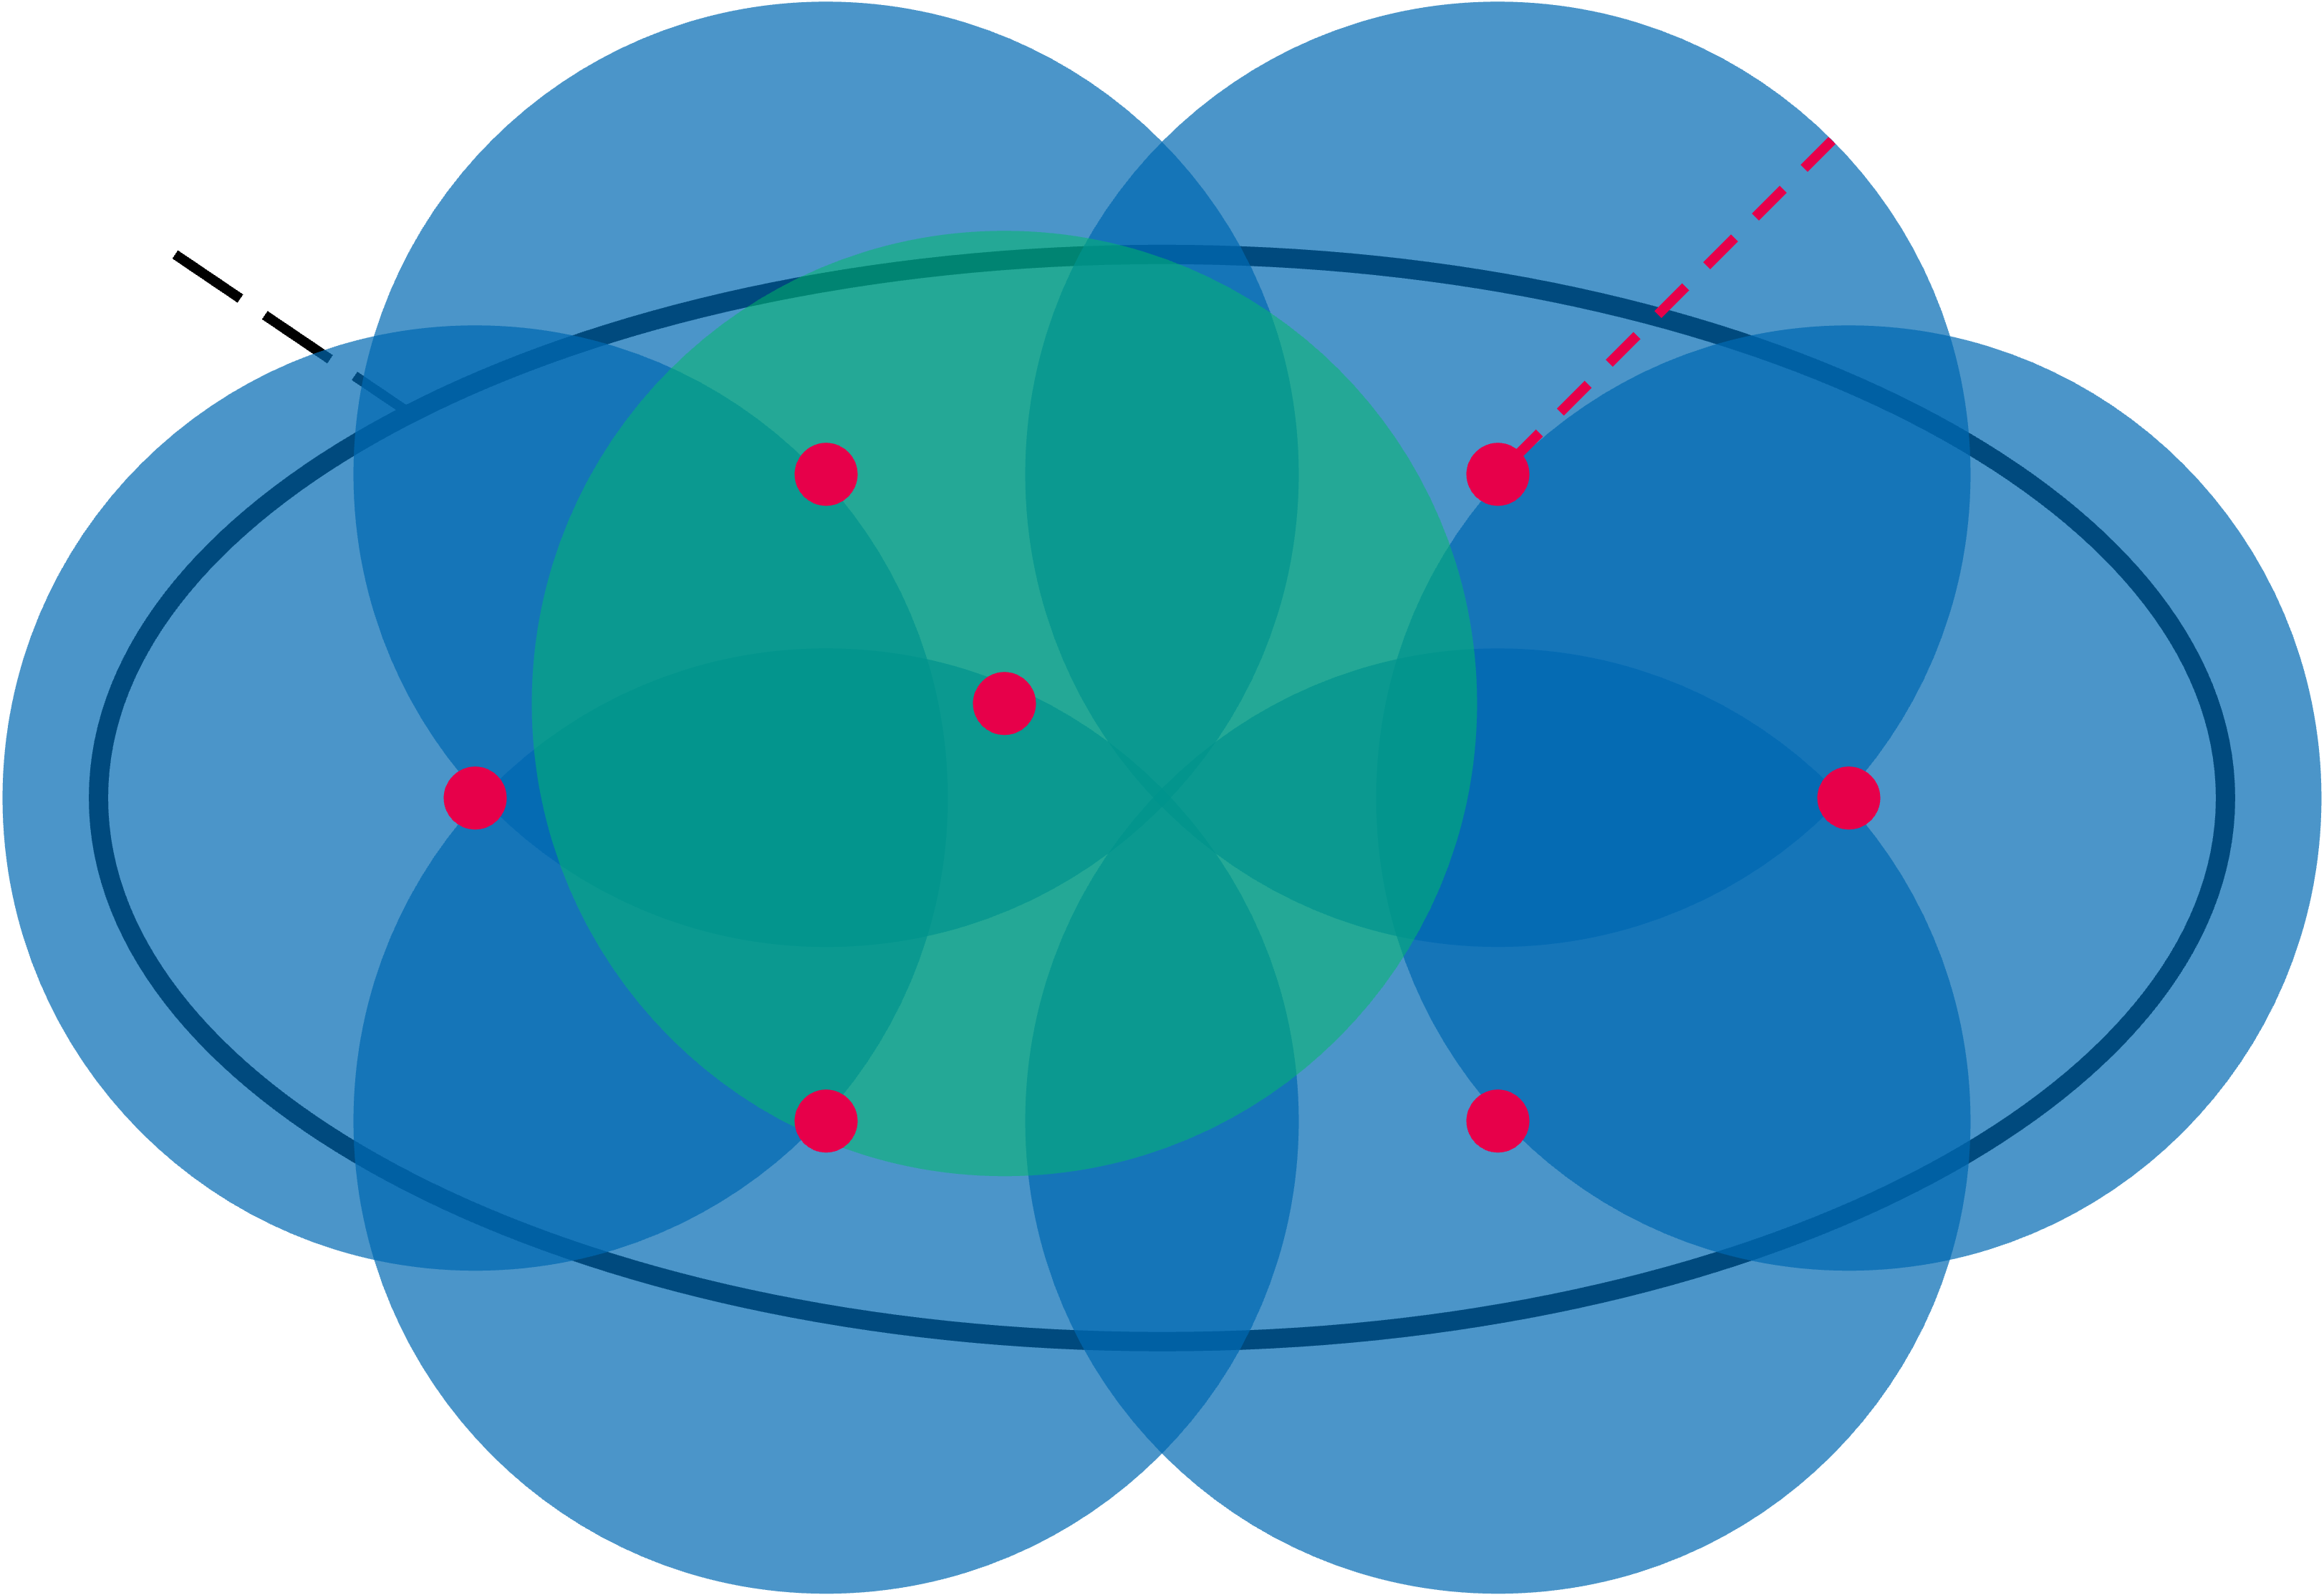
\includegraphics[width=10cm]{other/epsilon-net}
        };

        % Create scope with normalized axes
        \begin{scope}[
            x={(image.south east)},
            y={(image.north west)}]
         
            % Grid to properly align annotations
            % \draw[help lines, step=0.1] (image.south west) grid ($(image.north east) + (0.001,0)$);

            % Annotate image
            \node[] at (0.08,0.84) {$\mathcal{F}$};
            \node[] at (0.74,0.90) {$\varepsilon$};
            \node[] at (0.18,0.46) {$g_1$};
            \node[] at (0.33,0.26) {$g_2$};
            \node[] at (0.62,0.26) {$g_3$};
            \node[] at (0.77,0.46) {$g_4$};
            \node[] at (0.62,0.66) {$g_5$};
            \node[] at (0.33,0.66) {$g_6$};
            \node[] at (0.40,0.52) {$g_7$};
            
        \end{scope}
    \end{tikzpicture}
    \caption{%
         A class $\mathcal{F}$ covered by an $\varepsilon$-net ${\color{red} V} = \set{{\color{red} g_1}, \dots, {\color{red} g_7}}$. Note, however, that $N(\mathcal{F}, d, \varepsilon) < 7$ since the $\varepsilon$-ball centered on $g_7$ and depicted in green is redundant (i.e., the remaining 6 $\varepsilon$-balls still cover all of $\mathcal{F}$).
    }
    \label{fig: epsilon-net}
\end{figure}
